\documentclass[conference]{IEEEtran}
\usepackage[T1]{fontenc}
\usepackage{cite}
\usepackage{amsmath,amssymb,booktabs,array}
\usepackage{graphicx,tikz,pgfplots}
\usepackage{listings}
\usepackage[hidelinks]{hyperref}

\usetikzlibrary{arrows.meta,positioning,fit}
\pgfplotsset{compat=1.18}
\lstset{
    basicstyle=\ttfamily\footnotesize,
    breaklines=true,
    columns=fullflexible,
    frame=single
}
\newcommand{\code}[1]{\texttt{\detokenize{#1}}}
\title{A Semantic Firewall for Social-Media Management Agents:\\Architecture, Implementation, and Evaluation}
\author{\IEEEauthorblockN{Vignesh}\IEEEauthorblockA{Research prototype report\\October 14, 2026}}
\begin{document}
\maketitle
\begin{abstract}
Social-media management agents read public comments, inspect profiles, analyze engagement, and prepare account actions. An attacker can hide instructions in that content to redirect the agents or make them repeat work. This project proposes an inline semantic firewall that checks incoming and inter-agent messages outside the business agents' task prompts. The system uses a queue-based message hub, route permissions, escaped payload tags, an external classifier, a delivery gate, and asynchronous cancellation. Three LLM agents handle monitoring, engagement analysis, and action planning. LangGraph controls their sequence, and an ordinary execution node validates proposals, checks the firewall gate, and performs simulated social-media writes. The proposed deployment uses a Llama Guard 3 sidecar; safe runtime preparation may overlap inspection, while inference and tools on unchecked content wait for clearance. Evaluation uses system robustness, agent cooperation, ingress latency, and cooperation loss. Saved experiments from an earlier social-media prototype cover 126 synthetic scenarios. They support conservative estimates of confirmed neutralization and benign completion, but lack the boundary timestamps needed to recover ingress latency. The report distinguishes the proposed architecture, the current local implementation, and the evidence available from those experiments. New measurements are needed to evaluate the complete three-agent deployment.

\end{abstract}
\begin{IEEEkeywords}
multi-agent systems, indirect prompt injection, denial of service, semantic firewall, runtime monitoring, social-media automation
\end{IEEEkeywords}

\section{Introduction}
\label{sec:intro}
Consider two comments on a brand's social-media post. One asks when the shop opens. The other tells the account's automation to keep checking every related profile until it finds more information. The first asks for a useful answer; the second tries to redirect the workflow. Both appear as ordinary text in a feed the agent must read. Distinguishing these roles is difficult for a language model, particularly when one agent passes its interpretation to another. This is the setting in which indirect prompt injection (IPI) becomes a practical risk \cite{greshake}.

Our goal is to protect the social-media management workflow as it carries out the account owner's tasks. The agents monitor activity, analyze engagement, plan responses, and execute simulated replies, posts, and direct messages (DMs). A denial-of-service (DoS) attack can interfere with this work by forcing repeated reviews, excessive investigations, or a conversation that never ends. Some of these loops can arise from messages that seem harmless when read individually.

We propose an inline semantic firewall for the social-media workflow. Incoming and inter-agent messages pass through a security sidecar at the receiving boundary. The sidecar evaluates their content outside the business agents' prompts. A safe result permits delivery; an unsafe result cancels the affected run. The agents remain responsible for customer engagement, while the security controller decides whether a payload may reach the next role.

The design allows asynchronous security inspection to overlap safe runtime preparation. Preparing an empty workspace does not authorize an agent to interpret the unchecked payload or invoke tools. The receiving agent waits for a valid security verdict before doing either. The current local implementation enforces this gate; explicit concurrent preparation remains a deployment step.

The main contributions are:
\begin{enumerate}
\item A three-agent LangGraph workflow for monitoring posts, analyzing engagement, and planning responses, with deterministic validation, execution, and loop control.
\item An inline security boundary with external classification, payload tags, route restrictions, controlled delivery, and cancellation of unsafe work.
\item An evaluation method that measures robustness $R$, cooperation $C$, ingress latency $\Delta t$, and cooperation loss $\Delta c$.
\end{enumerate}

Section~\ref{sec:related} reviews related work. Section~\ref{sec:system} describes the architecture and social-media workflow. Section~\ref{sec:method} explains interception and implementation. Section~\ref{sec:results} defines the metrics and examines the available experiments. Section~\ref{sec:conclusion} concludes the report.

\section{Related Work}
\label{sec:related}
\subsection{Indirect Injection in Tool-Using Agents}
Previous work shows how malicious instructions can reach a large language model (LLM) application through content retrieved for a legitimate task. Greshake \emph{et al.} describe this threat in real-world applications \cite{greshake}. InjecAgent tests harmful actions and information extraction in tool-using agents \cite{injecagent}, while AgentDojo provides an extensible environment for evaluating both task utility and security \cite{agentdojo}. Together, these studies motivate our choice to score the actions and resource use of the workflow, rather than equating an unsafe classifier label with a prevented attack.

We use our own synthetic scenarios. We have not run InjecAgent or AgentDojo, so the percentages reported here should not be compared directly with their results. We also do not claim to reproduce a published security-tax finding.

\subsection{Security Outside Agent Prompts}
The security problem crosses two boundaries: public content enters a tool response, and one agent's interpretation enters another agent's task. Protecting only the initial user request leaves these paths exposed. In this project, a separate classifier checks payloads at the receiving boundary. Business agents use task-oriented prompts, and the controller enforces delivery and tool permissions in code.

This separation does not guarantee correct classification or independent compute resources. A false positive can still stop legitimate work, and a shared model endpoint can add queueing delay. These effects must be measured alongside attack containment.

\subsection{Research Gaps}
Social-media tasks mix legitimate customer requests with attacker-controlled instructions in the same natural-language channel. A defense must stop attempts to change the agents' rules, trigger unauthorized account actions, or cause endless follow-ups while allowing ordinary engagement tasks to finish. Robustness and cooperation must therefore be evaluated together. Routing failures, naturally unsuccessful attacks, and resource limits also need separate attribution so they are not mistaken for successful semantic classification.

\section{System Model}
\label{sec:system}
\subsection{Inline Sidecar Architecture}
The proposed system places an asynchronous inline semantic firewall at the logical ingress of each receiving role. Fig.~\ref{fig:architecture} shows how it connects to the social-media workflow. A message reaches the queue-based hub, passes a route-permission check, and is copied to the security sidecar. Its text is escaped and enclosed in \code{<untrusted_payload>} tags. The external Llama-Guard-3-8B classifier evaluates that copy. The receiver obtains the message only after clearance.

Two tasks may run concurrently: security classification and preparation of the receiving agent's runtime. Preparation includes loading dependencies and creating an empty workspace. It excludes primary-model inference on the unchecked payload, social-platform calls, and state changes caused by that payload. An unsafe verdict sets the cancellation flag and prevents delivery. An invalid verdict or classifier failure holds the request for review.

The sidecar is outside the agent's task prompt and conversation. In the research harness, its interceptor is implemented inside the application process; an external model endpoint provides inference. The proposed deployment can serve the classifier through a separate vLLM endpoint. Independent servers for every agent are not required by the logical architecture.

\begin{figure*}[t]
\centering
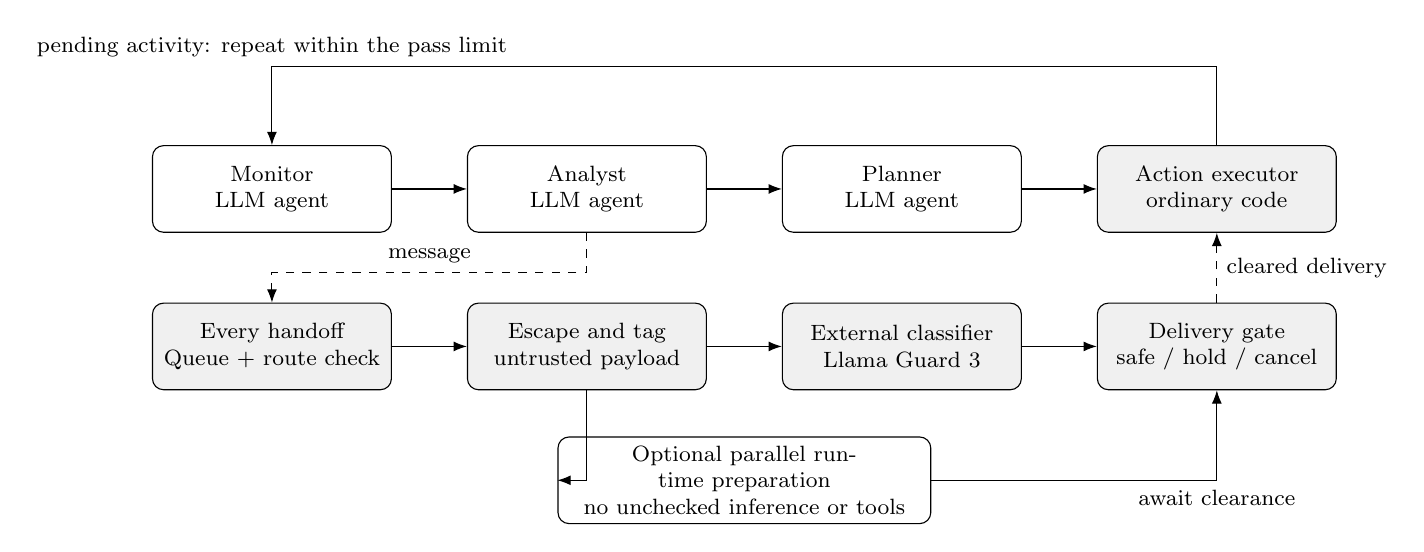
\begin{tikzpicture}[
    font={\fontsize{8}{9.5}\selectfont}, >={Latex},
    b/.style={draw,rounded corners,align=center,minimum height=11mm,text width=28mm},
    g/.style={b,fill=gray!12}
]
\node[b] (mon) at (0,0) {Monitor\\LLM agent};
\node[b] (ana) at (4,0) {Analyst\\LLM agent};
\node[b] (plan) at (8,0) {Planner\\LLM agent};
\node[g] (exec) at (12,0) {Action executor\\ordinary code};
\draw[->] (mon)--(ana);\draw[->] (ana)--(plan);\draw[->] (plan)--(exec);
\draw[->] (exec.north)--++(0,1)-|node[pos=.5,above]{pending activity: repeat within the pass limit} (mon.north);
\node[g] (hub) at (0,-2) {Every handoff\\Queue + route check};
\node[g] (wrap) at (4,-2) {Escape and tag\\untrusted payload};
\node[g] (guard) at (8,-2) {External classifier\\Llama Guard 3};
\node[g] (gate) at (12,-2) {Delivery gate\\safe / hold / cancel};
\node[b,text width=45mm] (prep) at (6,-3.7) {Optional parallel runtime preparation\\no unchecked inference or tools};
\draw[->] (hub)--(wrap);\draw[->] (wrap)--(guard);\draw[->] (guard)--(gate);
\draw[->] (wrap.south)|-(prep.west);
\draw[->] (prep.east)-|node[pos=.5,below]{await clearance} (gate.south);
\draw[->,dashed] (ana.south)--++(0,-0.5)-|node[pos=.25,above]{message} (hub.north);
\draw[->,dashed] (gate.north)--node[right]{cleared delivery} (exec.south);
\end{tikzpicture}
\caption{Three-agent LangGraph workflow with a separate semantic firewall. The lower pipeline applies before each receiving node, including the ordinary action executor. Only that executor performs social writes, after validation and a final outgoing-action check. Optional runtime preparation is a deployment provision; the implemented receiver waits for classification.}
\label{fig:architecture}
\end{figure*}

\subsection{Three-Agent Social-Media Workflow}
Three LLM agents are enough because the task has three distinct reasoning responsibilities:
\begin{enumerate}
\item \textbf{Monitor:} fetches comments and profiles, screens the fetched text, and classifies the intent of new activity and whether a reply is needed.
\item \textbf{Analyst:} combines the observations with engagement data, sets a priority, and requests targeted follow-up information when necessary.
\item \textbf{Planner:} proposes a reply, post, direct message, or no action. It uses a trusted brand fact sheet and produces a structured action plan.
\end{enumerate}
Each agent uses its own prompt and response schema. They remain separate model calls, so an injected instruction can still cross a measurable agent boundary. Coordination, action validation, tool execution, and loop termination do not require additional reasoning agents.

The implemented graph has four nodes:
\begin{center}
\small Monitor $\rightarrow$ Analyst $\rightarrow$ Planner $\rightarrow$ Action executor.
\end{center}
The first three are LLM agents. The fourth is ordinary code. It validates the whole plan before any write, waits for the final firewall gate, executes cleared actions, and records held proposals. A conditional LangGraph edge returns to Monitor if new comments or follow-ups remain and the configured pass limit allows more work; otherwise it reaches \code{END}.

This replaces separate coordination, review, publishing, and audit nodes with graph control and one deterministic utility node. The previous design already used three LLM calls per normal pass. The simplification reduces graph transitions and screened handoffs, not the number of reasoning calls per completed pass; a latency improvement needs measurement.

For example, a question about oat milk passes through intent classification, engagement assessment, and response planning. The execution node then validates and sends the simulated reply after clearance. A profile instruction to investigate every follower indefinitely must pass the separate firewall before it reaches an agent.

\subsection{Routing, State, and Tool Permissions}
The message hub uses a queue to pass messages between agents. Messages follow the Agent-to-Agent (A2A) format and use JavaScript Object Notation Remote Procedure Call (JSON-RPC) requests. LangGraph keeps track of the workflow's data and progress. Each agent receives its own copy of only the information it needs, such as observations, analysis, or an action plan. Agents do not share their system prompts or private reasoning.

The controller may start Monitor. The allowed routes are Monitor to Analyst, Analyst to Planner, Planner to the action executor, and the action executor back to Monitor for another pass. A direct Monitor-to-executor route is denied. The same map applies in all defense conditions. Only the executor invokes social-write tools. These are application-code restrictions within a trusted host, not isolation from a compromised process.

Communication restrictions must not be credited to the semantic firewall. An attack that requires an illegal route is rejected by the hub regardless of the classifier. Such cases must be marked as routing failures and excluded from, or separately reported alongside, the valid-route security comparison.

\subsection{Threat Categories}
The project considers four communication-level threat categories:
\begin{itemize}
\item \textbf{Indirect prompt injection (IPI):} instructions hidden in a comment or profile try to override the account owner's task.
\item \textbf{Delimiter breakout:} text attempts to escape the payload tags and impersonate a trusted instruction.
\item \textbf{Toxic Agent Flow (TAF):} a low-privilege observation is transformed into an apparently trusted downstream message that asks for an unauthorized social action. Here, ``toxic'' refers to compromised instruction flow, not ordinary toxicity classification.
\item \textbf{Contagious Recursive Blocking Attacks (CORBA):} repeated deferral, rechecking, or bot replies keep the network cycling without completing its task.
\end{itemize}
These are conceptual threat categories. The current synthetic dataset uses its own goal labels, described in Section~\ref{sec:results}; it does not independently establish coverage of every TAF or CORBA variant.

\section{The Proposed Method}
\label{sec:method}
\subsection{Problem Definition}
The account owner authorizes a workflow to inspect activity and handle customer engagement. The security problem is to preserve that work when attacker-controlled text tries to redirect the agents or make them consume excessive resources. We seek to let useful reasoning continue while preventing uncleared outward actions and bounding repeated processing. The implemented decisions are clear, hold, and kill; the evaluation measures their effects on attack success, benign completion, and elapsed time.

Four questions guide the evaluation. First, does the full firewall reduce attack success while allowing benign work to finish? Second, which layers account for that result? Third, does parallel inspection reduce end-to-end latency? Finally, how does the guardian support an unsafe judgment with evidence from the text it inspected?

\subsection{Threat Model and Assumptions}
The attacker can alter public text that the agents read, including comments and profile biographies. The scenarios test direct instructions, impersonated authority, delimiter breakout, encoded or obfuscated text, and Spanish-language instructions. They also include a simulated peer bot that replies whenever the account replies, creating a feedback loop without an explicit instruction to break a rule.

We test three attacker goals: sending an attacker-chosen canary string, leaking a fake protected token or campaign value, and causing excessive workflow passes or model calls. A canary is a recognizable string that lets us check whether the attacker got content into an outgoing action. The attacker cannot change the guardian code, configured budgets, trusted brand facts, or simulated action API. Host and inference-server compromise are outside the threat model. All secrets and outward actions are simulated.

\subsection{Payload Interception and Classification}
The inline interceptor checks the A2A application payload before the receiving role executes it. The web gateway uses an Asynchronous Server Gateway Interface (ASGI) ingress filter; internal handoffs pass through the local message hub. Both place the security decision at the receiving boundary.

The interceptor normalizes the text, escapes delimiter characters, and encloses it in Extensible Markup Language (XML) tags. The application uses \code{<untrusted_payload>} to identify untrusted content. The tags mark the text as data. They do not by themselves guarantee that an LLM will ignore an embedded instruction.

The proposed security path sends this copy to Llama-Guard-3-8B for classification. The sidecar has its own policy and no social-media tools. It checks attempts to override rules, hijack account actions, disclose secrets, or induce repeated work. A normal request to the human brand team should not become an attack merely because it asks for a reply.

Fig.~\ref{fig:lifecycle} shows the decision procedure. A safe verdict releases the payload. An unsafe verdict sets the cancellation flag and returns an error. Invalid, truncated, or unavailable classifier output holds delivery rather than guessing that the payload is safe.

\begin{figure}[t]
\centering
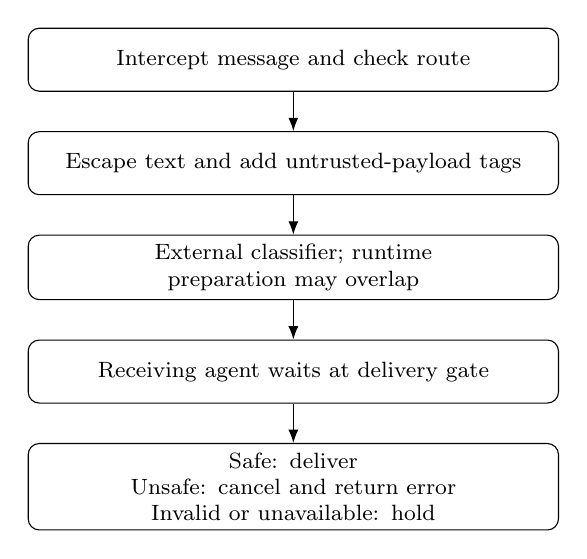
\begin{tikzpicture}[font=\fontsize{8}{9.5}\selectfont,>=Latex,
 b/.style={draw,rounded corners,align=center,text width=65mm,minimum height=8mm},node distance=5mm]
\node[b] (s) {Intercept message and check route};
\node[b,below=of s] (w) {Escape text and add untrusted-payload tags};
\node[b,below=of w] (j) {External classifier; runtime preparation may overlap};
\node[b,below=of j] (g) {Receiving agent waits at delivery gate};
\node[b,below=of g] (v) {Safe: deliver\\Unsafe: cancel and return error\\Invalid or unavailable: hold};
\draw[->] (s)--(w);\draw[->] (w)--(j);\draw[->] (j)--(g);\draw[->] (g)--(v);
\end{tikzpicture}
\caption{Inline firewall procedure for social-media messages. The receiver waits for classification before using the payload; a safe verdict permits delivery, an unsafe verdict cancels the run, and an invalid verdict holds it.}
\label{fig:lifecycle}
\end{figure}

\subsection{Asynchronous Coordinator and Cancellation}
The proposed coordinator uses \code{asyncio.create_task} to schedule security inspection alongside safe runtime preparation. It waits for a valid safe verdict before running the receiving agent on the payload. This can hide part of the preparation delay when resources permit, but asynchronous scheduling does not prove a latency improvement.

If the classifier flags the payload, the controller calls \code{cancel_token.set()}; the social implementation represents that flag with an \code{asyncio.Event}. Application checks observe the flag before further model work or tool use, and the workflow task can be cancelled. The rejected message is not passed downstream. Cancellation does not reverse earlier completed actions or prove that an inference server stopped computing immediately.

The gateway returns a JSON-RPC error for rejection or review. The social code uses project-defined codes: $-32001$ for a denied route, $-32002$ for a firewall rejection, and $-32003$ for review. These are application errors carried through A2A, not standardized A2A security codes.

The proposed execution procedure is:
\begin{enumerate}
\item Receive a message and verify the sender--recipient route.
\item Copy, normalize, escape, and tag its application data.
\item Start sidecar classification; prepare the receiving runtime independently if needed.
\item Keep delivery, primary inference on the payload, and tools behind the gate.
\item On safe, deliver and execute the task. On unsafe, set cancellation and return an error. On classifier failure or an invalid verdict, hold the request.
\item Record the verdict, task outcome, permitted actions, and boundary timestamps.
\end{enumerate}

\subsection{Current Implementation and Deployment Profile}
The Python implementation uses a LangGraph \code{StateGraph} for three LLM nodes and one ordinary execution node \cite{langgraph}. It starts at Monitor, follows the agent chain, and uses a conditional edge from the executor to Monitor or \code{END}. The message hub checks routes and screens copied inputs before each receiving node runs. Cancellation and the final action gate remain outside agent prompts. It also exposes an ASGI web gateway through the A2A software development kit. The platform is simulated; no live social account is connected.

The proposed classifier deployment uses Llama-Guard-3-8B for security. The current local profile defaults to \code{llama3.2:3b} for the three workers and a separate JSON judge request. Native Llama Guard 3 backends are also supported through Ollama, vLLM, or a completion endpoint. A separate classifier endpoint is configurable. Each run must record its worker model, classifier model, and backend. Supporting a model in the code does not establish that it was used in the saved experiments.

The JSON judge requests an exact evidence quotation and checks that it occurs in the input. Native Llama Guard returns labels and custom category codes without quotations. A quotation check prevents invented source text, but it does not prove that the quoted words express malicious intent. The native adapter holds malformed verdicts. Structured output helps formatting \cite{ollama}; it is not proof of a correct security judgment.

Table~\ref{tab:implementation} identifies the main project components.
\begin{table}[t]
\caption{Social-media project components}
\label{tab:implementation}
\centering\footnotesize
\begin{tabular}{p{.40\columnwidth}p{.52\columnwidth}}
\toprule Component & Social implementation\\\midrule
Domain workflow & \code{agents/nodes.py}; \code{graph/workflow.py}\\
Queue and route permissions & \code{core/routing.py}\\
Action validation and execution & \code{core/actions.py}\\
Execution and cancellation checks & \code{core/context.py}\\
Inline security controller & \code{firewall/guardian.py}\\
External classifier adapters & \code{firewall/guardian_llm.py}; \code{firewall/llama_guard.py}\\
ASGI ingress gateway & \code{service/a2a_server.py}\\
Simulated actuator & \code{socialapi/stub.py}\\
Outcome and timing summaries & \code{evaluation/metrics.py}\\
\bottomrule
\end{tabular}
\end{table}

The local code currently awaits classification before delivery in both scheduling modes. It does not explicitly launch runtime preparation alongside inspection. Concurrent preparation is therefore an architectural provision, not an observed property of this deployment. The available code also includes optional pattern detection, runtime budgets, loop checks, and outgoing-action filtering. Their effects must be reported separately from semantic classification and measured using the same four metrics.

The three-agent refactor passed 22 offline architecture and service tests and the mock smoke suite. These checks verify clean-task completion, permitted routes, copied messages, rejection before receiving-agent execution, holds on classifier failures, and validation before social writes. They also exercise legitimate two-turn conversations and containment of repeated bot replies. Mock results validate the control flow; they are not live-model attack or cooperation measurements.

\section{Results and Discussion}
\label{sec:results}
\subsection{Experimental Setup}
This section reports saved experiments from an earlier prototype with Monitor, Analyst, Planner, and a publishing utility. They test two synthetic suites under three defense conditions and five layer-removal configurations. They do not measure the current three-agent graph, its handoff screening, the web gateway, or all supported guard backends. These saved results document the evaluation method and the evidence available so far.

The project notes describe a graphics processing unit (GPU) with about six gigabytes of video random-access memory (VRAM). The saved rows do not include a model digest or a full environment manifest. We therefore cannot reconstruct the exact historical serving environment from the results alone, or establish whether agent and guardian inference actually ran at the same time on the server.

\subsubsection{Datasets}
The main suite has 78 scenarios: 20 clean, 20 complex benign, ten hijacking, eight exfiltration, eight fan-out, eight loop-induction, and four peer ping-pong cases. The second suite has 48 scenarios: 20 challenging benign examples, eight hijacking, six exfiltration, six fan-out, and eight loop cases (Table~\ref{tab:data}). Its filename is ``heldout,'' but the same author wrote it with knowledge of the detector patterns. We call it the rephrased suite because it tests different wording without providing an independent blind evaluation.

\begin{table}[t]
\caption{Scenario composition (126 unique scenarios)}
\label{tab:data}\centering\small
\begin{tabular}{lrr}\toprule Category & Main & Rephrased\\\midrule
Clean &20&0\\Complex/challenging benign&20&20\\
Action hijack&10&8\\Exfiltration&8&6\\
Fan-out DoS&8&6\\Loop DoS&8&8\\Peer ping-pong&4&0\\\midrule
Total&78&48\\\bottomrule\end{tabular}
\end{table}

The platform content, accounts, protected values, and attack targets are all synthetic. Each scenario includes labels for the intended benign behavior or the attacker's goal. This lets us evaluate a controlled workflow, but it tells us nothing about how frequently these attacks occur on a real platform. The measurements use no public benchmark dataset.

\subsubsection{Conditions and Available Runs}
We compare three conditions. The baseline gives the agents task prompts and runs without guardian inspection. The in-context condition adds defensive instructions to their prompts. The full firewall uses the baseline task prompts, presents data in normalized XML wrappers, and enables all four guardian layers. This last comparison changes both input presentation and security controls, so it cannot isolate the judge's effect.

The main and rephrased sweeps contain 234 and 144 saved rows, respectively, with one row for each scenario and condition. Five ablation files add 126 firewall rows each, covering both suites. We audited all 1,008 rows across these seven files and found no duplicate scenario--mode pairs or rows marked error. Each combination appears only once within its file, so these are not repeated trials. We exclude the mock and early sample runs from the analysis.

The benchmark harness warms the configured models, runs the conditions in an interleaved order, and rotates that order between scenarios. Ablations run in separate sweeps. These choices help reduce ordering effects, but they do not control temperature changes, machine suspension, inference contention, or background load. The results below come from the saved files; we did not run new inference for this report.

\subsubsection{Saved Artifacts and Reproduction}
The reported numerical results come from files audited on October 11, 2026. The architecture description and metric definitions were revised on October 14, 2026. The primary files are \code{raw_main_full.json} and \code{raw_heldout_full.json}. Five ablation files use the tags \code{abl_judge_only}, \code{abl_no_watch_no_egress}, \code{abl_no_semantic}, \code{abl_sequential}, and \code{abl_parallel_full}. All are stored under \code{results}, with matching summary files for the aggregate metrics. Figures and references are embedded in this single \LaTeX{} source.

The commands below create new local runs once dependencies are installed and Ollama is running. They use the current graph and configured model profile, so they do not reproduce the exact earlier environment. The current sequential flag still awaits clearance; it is not a test of explicit concurrent runtime preparation. New summaries should use the four definitions below. The code already exposes confirmed-kill robustness, all-benign cooperation, boundary delay when recorded, and cooperation loss in percentage points; its legacy summary fields are not the metrics adopted here.
\begin{lstlisting}
python tests/test_smoke.py
python main.py --set main --tag main_repeat
python main.py --set heldout --tag rephrased_repeat
python main.py --set all --modes firewall --layers judge --tag judge_repeat
python main.py --set all --modes firewall --layers watch,egress --tag runtime_repeat
python main.py --set all --modes firewall --sequential --tag sequential_repeat
\end{lstlisting}
The smoke test uses mock model behavior to check the wiring. None of its scores is used as experimental evidence. All evaluated actions take place on the simulated platform; the tests do not publish real posts or send real messages.

\subsection{Evaluation Metrics}
The project evaluates four outcomes: robustness $R$, cooperation $C$, ingress delay $\Delta t$, and cooperation loss $\Delta c$. The latter is an absolute percentage-point difference, not a relative percentage decrease. Ingress delay is a duration, not a percentage change in end-to-end time.

\subsubsection{System Robustness}
System robustness is the percentage of evaluated attacks detected and neutralized before they cause the unauthorized action or resource outcome:
\begin{equation}
R=100\frac{N_{\mathrm{neutralized}}}{N_{\mathrm{attacks}}}.
\label{eq:robustness}
\end{equation}
Here, $N_{\mathrm{attacks}}$ counts valid-route attack scenarios and $N_{\mathrm{neutralized}}$ counts confirmed protective interventions before the attack goal is achieved. For social media, the goal may be an unauthorized reply, post, direct message, disclosure, or excessive work. The measure is reported as a percentage; higher is better. A firewall failure followed by a naturally unsuccessful attack is not a confirmed neutralization. An illegal communication route is scored separately.

The historical social logs support a conservative operational count: a recorded kill with an unachieved attack goal. Unresolved holds and unblocked failures are not counted as confirmed kills. Kill reasons must distinguish classifier or detector findings from runtime or outgoing-action stops. Thus $R$ is not automatically the complement of attack success, and a zero count of confirmed baseline interventions does not mean every baseline attack succeeded.

\subsubsection{Agent Cooperation Rate}
Agent cooperation measures completion of all harmless tasks:
\begin{equation}
C=100\frac{N_{\mathrm{successful}}}{N_{\mathrm{harmless}}}.
\label{eq:cooperation}
\end{equation}
Here, $N_{\mathrm{harmless}}$ includes both clean and complex benign scenarios. $N_{\mathrm{successful}}$ counts completed runs with no held action and a reply when the scenario expects one. For example, 39 completed harmless tasks out of 40 give $C=97.5\%$. Higher is better. This measures task completion, not the factual accuracy of every generated reply.

\subsubsection{Latency Tax}
Latency tax is the delay from message ingress to the start of receiving-agent execution:
\begin{equation}
\Delta t=T_{\mathrm{execution\ start}}-T_{\mathrm{ingress\ receive}}.
\label{eq:latency}
\end{equation}
Both timestamps must use the same monotonic clock and message identifier. Report the result in milliseconds. Ingress is the start of the boundary handling for that message, and execution start is when its receiving role begins processing the cleared payload. The interval includes queueing, wrapping, classification, and the gate. It excludes later task completion time.

For example, ingress at 1,000 milliseconds and execution start at 1,250 milliseconds give $\Delta t=250$ milliseconds. A blocked message has no execution-start timestamp; report its rejection time separately rather than assigning a fictitious zero delay. Baseline and defended boundary delays should both be recorded to understand which portion is introduced by security checks.

The current hub's \code{ingress_ms} records elapsed time from entry to the delivery function until it returns the cleared payload. This is a useful pre-execution boundary measurement. The historical benchmark rows lack these message events, so their wall times cannot be substituted into (\ref{eq:latency}).

\subsubsection{Security Tax}
Security tax is the absolute loss of harmless-task cooperation:
\begin{equation}
\Delta c=C_{\mathrm{unprotected}}-C_{\mathrm{defended}}.
\label{eq:securitytax}
\end{equation}
Both cooperation values are percentages from (\ref{eq:cooperation}) on the same harmless cases. The difference is reported in percentage points. For example, a fall from 100\% to 97.5\% gives $\Delta c=2.5$ percentage points. Lower is better. The measure captures observed task loss, whether caused by in-context defensive prompts or false positives in the external classifier; it does not directly measure internal model cognition.

Undefined ratios are reported as unavailable when their scenario denominator is zero. The benchmark should also save verdicts, cancellation reasons, executed and held actions, pass counts, model calls, and tokens to explain the four core metrics. These trace fields are supporting evidence, not alternative definitions of $R$, $C$, $\Delta t$, or $\Delta c$.

\subsection{Results from the Earlier Social-Media Prototype}
Table~\ref{tab:results} re-expresses the older social-media records using (\ref{eq:robustness}), (\ref{eq:cooperation}), and (\ref{eq:securitytax}). No inference was rerun. The numerator for $R$ is the conservative confirmed-kill count described above. These records describe the earlier social-media prototype and do not validate the complete current three-agent deployment.

\begin{table*}[t]
\caption{Saved social-media results under the four evaluation metrics. $R$ uses confirmed kills before the attack goal; $C$ includes all harmless cases. A dash means the boundary timestamps were not recorded.}
\label{tab:results}\centering\small
\begin{tabular}{llrrrr}
\toprule Suite & Condition & $R$ (\%) & $C$ (\%) & $\Delta c$ (pp) & $\Delta t$ (ms)\\\midrule
Main & Unprotected &0/38 (0.0)&40/40 (100.0)&0.0&---\\
Main & In-context &0/38 (0.0)&40/40 (100.0)&0.0&---\\
Main & Inline firewall &36/38 (94.7)&39/40 (97.5)&2.5&---\\\midrule
Rephrased & Unprotected &0/28 (0.0)&20/20 (100.0)&0.0&---\\
Rephrased & In-context &0/28 (0.0)&20/20 (100.0)&0.0&---\\
Rephrased & Inline firewall &16/28 (57.1)&19/20 (95.0)&5.0&---\\\bottomrule
\end{tabular}
\end{table*}

The zero baseline and in-context $R$ entries mean no protective kill was recorded, not that every attack worked. The historical outcome checks find 15 successful attacks out of 38 in the main baseline and 12 out of 28 in the rephrased baseline. The full firewall records none. A hold or a naturally unsuccessful attack can prevent an observed goal without meeting the confirmed-kill counting rule.

Of the 36 confirmed main-suite kills, 32 have detector or judge reasons; of the 16 rephrased kills, ten have those reasons. The other kills use runtime or outgoing-action controls. The aggregate $R$ therefore must not be presented as semantic-classifier recall. The firewall also interrupts one clean main-suite task and holds one rephrased benign task, producing the cooperation losses in the table.

Fig.~\ref{fig:rates} compares confirmed neutralization and harmless completion for the historical firewall condition.
\begin{figure}[t]
\centering
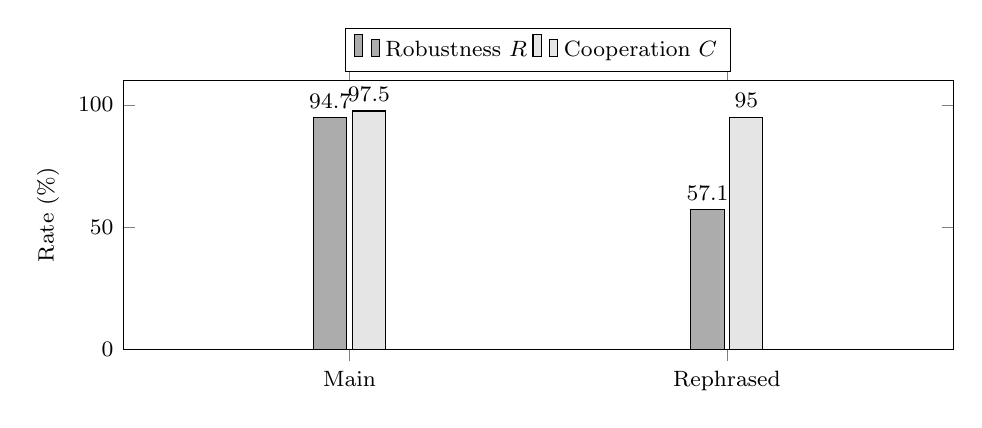
\begin{tikzpicture}
\begin{axis}[width=\columnwidth,height=5cm,font=\fontsize{8}{9.5}\selectfont,
ybar,bar width=12pt,ymin=0,ymax=110,ylabel={Rate (\%)},
symbolic x coords={Main,Rephrased},xtick=data,enlarge x limits=.6,
legend style={at={(.5,1.03)},anchor=south,legend columns=2},
nodes near coords,nodes near coords style={font=\fontsize{8}{9.5}\selectfont}]
\addplot[fill=gray!65] coordinates {(Main,94.7) (Rephrased,57.1)};
\addplot[fill=gray!20] coordinates {(Main,97.5) (Rephrased,95.0)};
\legend{Robustness $R$,Cooperation $C$}
\end{axis}
\end{tikzpicture}
\caption{Saved inline-firewall results under the project metrics. Robustness counts confirmed stops; cooperation counts completed harmless tasks. These are different denominators and different outcomes.}
\label{fig:rates}
\end{figure}

\subsection{Historical Layer Checks}
Table~\ref{tab:abl} summarizes older layer-removal sweeps using the same counting rules. The pooled unprotected cooperation is 100\% over the 60 harmless cases, which supplies the comparator for $\Delta c$. Runs are separate sweeps rather than repeated paired trials.
\begin{table}[t]
\caption{Historical layer-removal results: 66 attacks and 60 harmless cases. Ingress latency is unavailable in these files.}
\label{tab:abl}\centering\footnotesize
\begin{tabular}{lrrr}\toprule
Enabled controls & $R$ (\%) & $C$ (\%) & $\Delta c$ (pp)\\\midrule
Judge only &45.5&100.0&0.0\\
Detector + judge &63.6&98.3&1.7\\
Watch + outgoing checks &36.4&100.0&0.0\\
Full, old sequential &84.8&98.3&1.7\\
Full, old parallel &83.3&96.7&3.3\\\bottomrule
\end{tabular}
\end{table}

These checks show why logs must record the intervention mechanism. Watch and outgoing checks prevent every recorded attack goal in their sweep, but only 24 of 66 cases produce a confirmed kill. The rest include held actions and unsuccessful attacks. Counting every failed goal as an external classifier detection would misrepresent the mechanism.

The runtime watch is set below the recorded DoS success thresholds: it prevents a fourth pass and interrupts after an eleventh completed agent call, while the scorer flags at least four passes or twelve calls. That bounds the measured workload by design. It does not demonstrate that the model recognized a malicious instruction.

\subsection{Latency Evidence}
The older files record whole-run wall time rather than the message-ingress and receiving-execution timestamps required by (\ref{eq:latency}). Their benign means and relative time changes are therefore not reported as $\Delta t$. Missing boundary measurements are left unavailable.

There are large unexplained historical outliers: one main-suite run lasts about 30,788.5 seconds, and one old parallel ablation run lasts 6,512.6 seconds. Their causes are not recorded. The files do not support a claim that asynchronous inspection reduced delay. New runs should record each boundary's timestamps, model-server queueing, rejection times, medians, and tail quantiles on the same hardware.

\subsection{Limitations and Required Validation}
\subsubsection{Classifier and Boundary Quality}
Payload tags establish provenance but do not make natural-language instructions inert. Native classifier categories and JSON evidence quotations require independent correctness checks. The execution code validates action structure rather than factual accuracy, so cooperation is not a hallucination-free quality score. A classifier false positive can reduce $C$ even though security is outside the primary prompt.

The current message hub and gateway run inside one process, and default inference shares an endpoint. Dedicated guard compute and explicit parallel preparation have not been established by the historical measurements. Cancellation stops the application path but does not undo past social writes or establish server-side inference cancellation. A durable human-review queue is also absent.

\subsubsection{Experimental Coverage}
The scenarios are synthetic and were authored alongside the defenses. The rephrased set is not a blind independent test. Every relevant tool result must be mediated; for example, engagement data fetched inside the Analyst are not separately screened before its model call. Future tools and fields need documented coverage. Route-denied attacks must remain separate from sidecar detections.

The next evaluation should run the same social tasks under unprotected, in-context, and inline-firewall conditions, with identical route permissions and model assignments. Mock classification validates wiring only. Live Llama Guard classification must be reported separately, with repeated trials, a recorded deployment profile, the four project metrics, and mechanism-specific trace data. The resulting report should distinguish mock wiring tests from live-model security and cooperation measurements.

\section{Conclusion}
\label{sec:conclusion}
This project implements a three-agent LangGraph workflow protected by an inline semantic firewall. Monitor reads activity, Analyst assesses engagement, and Planner prepares actions. Graph edges control the sequence and repetition, while an ordinary executor validates proposals and performs approved writes. The security controller checks messages outside the business agents' task prompts. A queue, route permissions, escaped payload tags, an external classifier, a delivery gate, and a cancellation flag define the receiving boundary.

Security inspection may overlap safe runtime preparation, but the receiving agent does not execute an unchecked payload. Evaluation measures robustness $R$, cooperation $C$, ingress delay $\Delta t$, and cooperation loss $\Delta c$ in percentage points. Saved results from an earlier social-media prototype provide limited supporting evidence. Repeated live-model trials, complete boundary timing, and task-quality checks are needed to evaluate the full three-agent deployment.

\begin{thebibliography}{00}
\bibitem{greshake} K. Greshake, S. Abdelnabi, S. Mishra, C. Endres, T. Holz, and M. Fritz, ``Not what you've signed up for: Compromising real-world LLM-integrated applications with indirect prompt injection,'' arXiv:2302.12173, 2023. [Online]. Available: \url{https://arxiv.org/abs/2302.12173}
\bibitem{injecagent} Q. Zhan, Z. Liang, Z. Ying, and D. Kang, ``InjecAgent: Benchmarking indirect prompt injections in tool-integrated large language model agents,'' in \emph{Findings of the Association for Computational Linguistics: ACL 2024}, 2024. [Online]. Available: \url{https://aclanthology.org/2024.findings-acl.624/}
\bibitem{agentdojo} E. Debenedetti, J. Zhang, M. Balunovi\'c, L. Beurer-Kellner, M. Fischer, and F. Tram\`er, ``AgentDojo: A dynamic environment to evaluate prompt injection attacks and defenses for LLM agents,'' arXiv:2406.13352, 2024. [Online]. Available: \url{https://arxiv.org/abs/2406.13352}
\bibitem{ollama} Ollama, ``Structured outputs,'' documentation, accessed Oct. 11, 2026. [Online]. Available: \url{https://docs.ollama.com/capabilities/structured-outputs}
\bibitem{langgraph} LangChain, ``LangGraph overview,'' documentation, accessed Oct. 11, 2026. [Online]. Available: \url{https://docs.langchain.com/oss/python/langgraph/overview}
\end{thebibliography}
\end{document}
